\documentclass[tikz,border=3pt]{standalone}
\usepackage[utf8]{inputenc}
\usepackage[T1]{fontenc}
\usepackage{libertinus}
\usepackage{amsmath,amssymb}
\usetikzlibrary{arrows.meta,calc,patterns,decorations.pathmorphing,decorations.markings,decorations.pathreplacing,bending}
\definecolor{UGblue}{RGB}{0,51,102}
\newcommand{\dbar}{\mathchar'26\mkern-12mu d}
\tikzset{
  >=Stealth,
  every node/.style={font=\small},
  caja/.style={draw,line width=0.9pt},
  pared/.style={draw,line width=1.6pt},
  ejes/.style={->,line width=0.8pt},
  adia/.style={draw,pattern=north east lines,pattern color=black!70,line width=0.5pt},
  gas/.style={fill=UGblue!8},
  punto/.style={fill,circle,inner sep=1.3pt},
  onda/.style={decorate,decoration={snake,amplitude=1.1pt,segment length=5pt,post length=3pt,pre length=0pt}},
}
\begin{document}
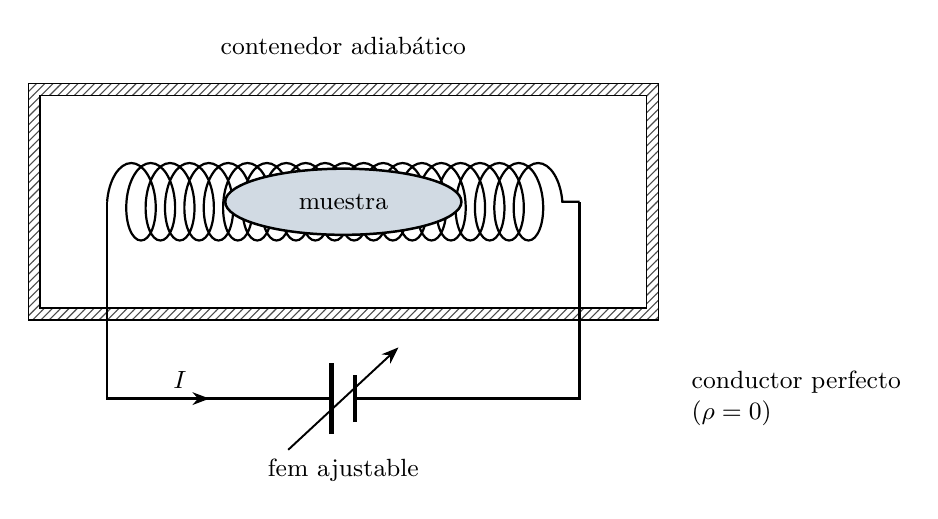
\begin{tikzpicture}
  % contenedor adiabático
  \filldraw[even odd rule,pattern=north east lines,pattern color=black!70,line width=0.5pt] (-1.0,-1.5) rectangle (7.0,1.5) (-0.85,-1.35) rectangle (6.85,1.35);
  % solenoide
  \draw[decorate,decoration={coil,aspect=0.5,segment length=7pt,amplitude=14pt},line width=0.8pt] (0,0) -- (6,0);
  % muestra
  \filldraw[fill=UGblue!18,draw=black,line width=0.9pt] (3,0) ellipse (1.5 and 0.42);
  \node at (3,0) {muestra};
  % cableado y batería
  \draw[line width=0.9pt] (0,0) -- (0,-2.5) -- (2.85,-2.5);
  \draw[line width=0.9pt] (3.15,-2.5) -- (6,-2.5) -- (6,0);
  \draw[line width=1.6pt] (2.85,-2.95) -- (2.85,-2.05);
  \draw[line width=1.6pt] (3.15,-2.8) -- (3.15,-2.2);
  \draw[->,line width=0.7pt] (2.3,-3.15) -- (3.7,-1.85);
  \node[below] at (3,-3.15) {fem ajustable};
  \draw[->,line width=0.7pt] (0.55,-2.5) -- (1.3,-2.5) node[midway,above] {$I$};
  \node[above,align=center] at (3,1.75) {contenedor adiabático};
  \node[right,align=left] at (7.3,-2.5) {conductor perfecto\\($\rho=0$)};
\end{tikzpicture}
\end{document}
